\chapter{Preliminaries and Problem Setup}
\label{sec:preliminariesProblem}


In the following chapter, the problem setup handled by the Master Thesis will be explained.
Further, preliminaries regarding assumptions and other decisions are defined.

\section{Reconstruction problem}
\label{sec:reconstructionProblemCT}
Tomographic reconstruction is a popular inverse problem \cite{tomographicReconstruction}. 
The aim is to reconstruct an object $x$ from its observed projections $P=[p_0, p_1, \dots, p_N]$.
More formally, the aim is to recover some density function $f$ from overserved samples $y$, taken from the line-integral $p(\cdot)$.

The problem can be defined as a two-dimensional (2D) problem but also as a three-dimensional (3D) problem. In the following, we focus on the 2D case.
In 2D, also called classical tomography reconstruct problem, the underlying density function is in two dimensions and the measurements lines lie on a plane.

The problem automatically gets harder, if we deal with incomplete datasets (subset of measured lines, limited angle data) but also with noisy observations.
Moreover, the angle $\theta$ of the projections are not always known.

\subsection{Computer tomography}

First of all, lets define the line integral $p$ of our unknown density function $f$ in the 2D case:

\begin{equation}
    \begin{aligned}
        p(\theta, s)   &=  R f(\theta, s) \\
        R f(\theta, s) &=  \int_{-\infty}^{\infty} f(x(z), y(z)) dz \\
                       &= \int_{-\infty}^{\infty} f((z \sin \theta + s \cos \theta), (-z \cos \theta + s \sin \theta)) dz \\
    \end{aligned}
\end{equation}

where $p$ is the line integral of the density function $f$, $\theta$ the projection angle and $s$ the distance from the origin.

In the 2D case, the line integral corresponds to the Radon-Transform \cite{radonTransform}.
When data of the line integral is presented as a 2D image, we are speaking from the \textit{sinogram}.
With the 2D Radon transform, we can map the density function $f$ to the sinogram $p$. 

%\begin{figure}
%    \centering
%    \subbottom[Radon Transform  $R f(\theta=45, s=0)$\label{fig:phantom_theta45}]{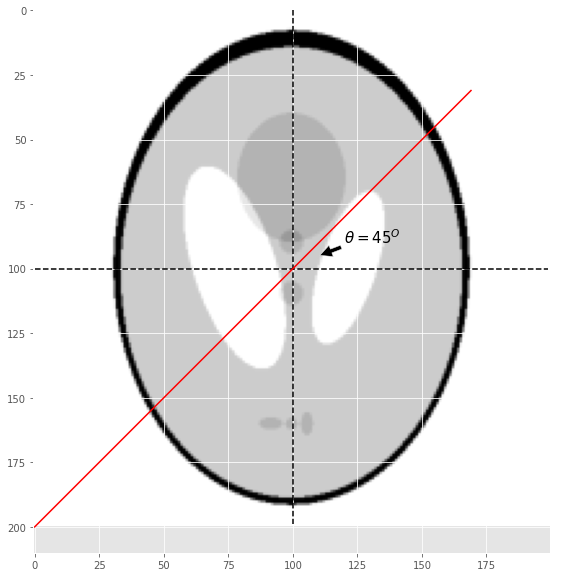
\includegraphics[width=0.3\textwidth]{phantom_theta45.png}}
%    \subbottom[Radon Transform  $R f(\theta=45, s=14.14)$\label{fig:phantom_theta45_s14}]{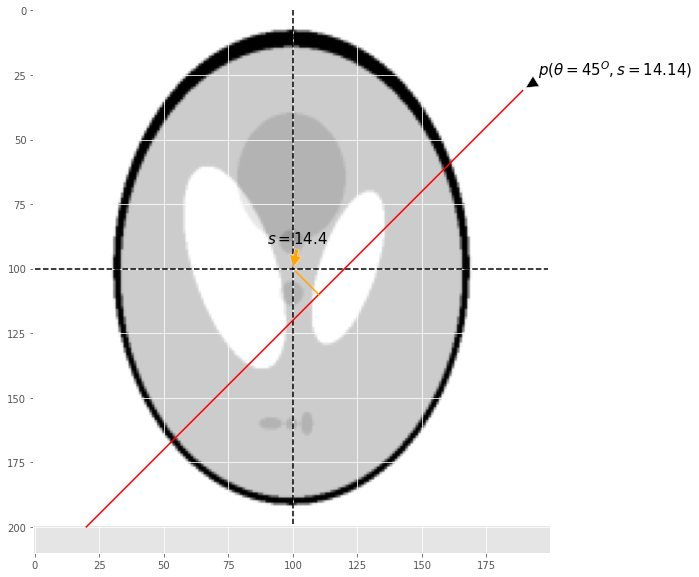
\includegraphics[width=0.3\textwidth]{phantom_theta45_s14.png}}
%    \subbottom[Shepp–Logan phantom sinogram of $p(\theta=45, s=0)$\label{fig:phantom_sinogram}]{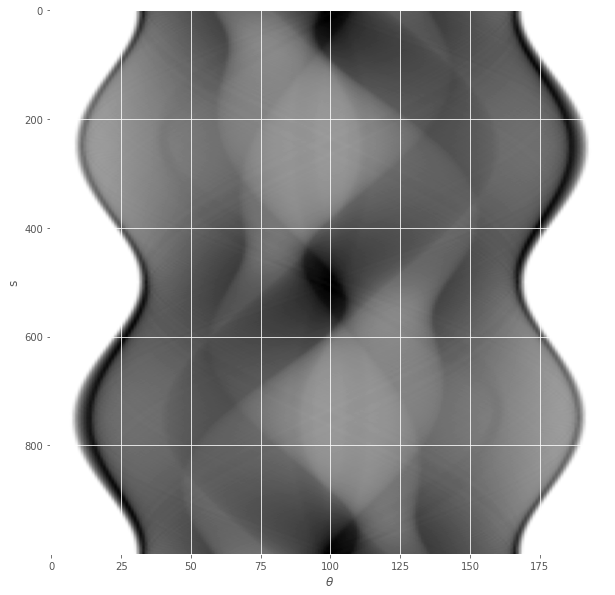
\includegraphics[width=0.3\textwidth]{phantom_sinogram.png}}
%    \caption{Examples, where the original object $x$ is the Shepp-Logan phantom.}
%    \label{fig:phantom}
%\end{figure}

\subsection{Filter Backprojection}
\label{sec:filterBackProjection}
Filter Backprojection (FBP) is a reconstruction method, which allows to solve for $p$. It is equivalent to the inverse of the Radon Transform
and is related to the Fourrier transform. Basically, it maps sinograms of $p$ back to the density function $f$.

The problem with the algorithm is, that it only works for complete data and without noise.



\section{Cryo-EM}


\subsection{Single particle multireference alignment (MRA)}


\subsection{Extension for PSF}

Why exactly?
Convolving (point spread function) PSF  with observation.


\section{General form}

In the following, we want to defined a form, which is valid for the 2D reconstruction 
problem of CT as well as the 3D cryo-EM problem.


\begin{equation}
    \begin{aligned}
        y_i &= g_i  A(x, \theta) + noise \\
    \end{aligned}
\end{equation}

where $y_i$ is the observed sample, $x$ our original object and $A(x, \theta)$ a non-linear operator.



\subsection{Extension}
Again, we can extend the formula to:

\begin{equation}
    \begin{aligned}
        y_i &= h_i \times g_i  A(x, \theta) + noise \\
    \end{aligned}
\end{equation}

\subsection{2D example}

$a_i \in SO(1)$
$A := N \times N$
$B := N$

$f(x) = \int_{\theta = 0}^{\pi} p(\theta, s) |_{s=x \cdot (- \sin \theta, cos \theta) } d \theta$



\subsection{3D example}

$a_i \in SO(2)$
$A := N \times N \times N$
$B := N \times N$



%The concept of Radon transform was extended as well and can be applied to higher dimensions as well.


\section{Manifold assumption}
In the reconstruct problem, we can apply the Manifold assumption from section \ref{sec:manifoldAssumption}.
Moreover, in the none-noisy case, we can even assume how this Manifold look like.

The manifold, and therefore, a low-dimensional embedding, can be calculated the following:

\begin{enumerate}
    \item Construct the knn-graph from our line integral (sinogram).
    \item Calculate the normalized Graph Laplacian
    \item Extract the second, third (and fourth) smallest eigenvectors
\end{enumerate}

\textbf{todo: Show with Shepp-Logan-phantom that we get unit-cirlce}

The showed example can be extended to 3D, where the underlying manifold corresponds to the Sphere.
Therefore, we can derive, that our angles have the following property:
In the 2D case, $\theta \in SO(1)$ and the in 3D case, $theta \in SO(2)$.

Again, the circle and sphere can be computed and for the none-noisy, the underlying Manifold can be seen as known.


\section{Thesis problem}
During the Master Thesis, the reconstruction problem with unknown angles is considered. 
Moreover, the observed samples are considered to be noisy. 

The resulting proposed algorithm should work in the 2D and 3D scenario.

The main idea is, to exploit the fact that the underlying Manifold is known (Circle in 2D and Sphere in 3D). 

From our noisy observations, we can compute the approximated manifold and compare it with the original manifold.
The comparison between the manifold enables the possibility of a Loss function and Learning in general.




Simple Case in 
